\chapter{Introduction}

\section{Introduction}
 
SEXTANTE is a platform for geospatial analysis which makes it easy to implement and use geoalgorithms. This programming guide is targeted at programmers who want to incorporate SEXTANTE--based capabilities into their sofware, and also at those who would like to implement new algorithms using the SEXTANTE framework.

To follow this guide, you must have a basic knowledge of the Java programming language. Knowledge of fundamental GIS concepts is also assumed. Examples are based on the Eclipse IDE, but they can be easily adapted to other development environments.

It is recommended to read the \emph{Introduction to SEXTANTE} document before reading this text. It  can be downloaded from the same website from which you downloaded this guide. Basic ideas about SEXTANTE are covered on that text and will not be included here.
 
 \section{Getting SEXTANTE}

Whether you want to add new algorithms to the SEXTANTE library or use those geoalgorithms already developed, you need to have SEXTANTE and add it to your project. From the SEXTANTE website you can download binary files, and the source code is available via the SVN repository. Using binary files is recommended, unless, of course, you want to extend the library and add new features (not necessarily new algorithms). 

%Chapter \ref{CompilingSextante} gives more information about how to use the SEXTANTE source code for these purposes.

The zip file that can be downloaded from the SEXTANTE website contains a folder named \texttt{core} which includes the following jar files. A short description of each of them is given, in order to explain the role it plays.

\begin{itemize}
 \item Base SEXTANTE files: these constitute the minimum set of files that you have to add to your project if you want to work with SEXTANTE.
\begin{itemize}
\item \texttt{sextante.jar}: SEXTANTE core classes.
\item \texttt{jts-1.12.jar} Java Topology Suite library, used to handle vector geometries.
\item \texttt{jcommons-1.0.0.jar}: Base elements for the JFreeChart library.
\item \texttt{jfreechart-1.0.1.jar}: JFreeChart library, used for generating charts as output of geoalgorithms.
\item \texttt{kxml2.jar}. XML library.
\item \texttt{libMath.jar}. Additional SEXTANTE library for mathematical operations.
\end{itemize}

\item Geoalgorithms: \texttt{sextante\_algorithms.jar}.

\item Graphical elements and dependencies.
\begin{itemize}
\item \texttt{sextante\_gui.jar}: SEXTANTE GUI elements.
\item \texttt{jgraph.jar}. Used for the graphical modeler interface.
\item \texttt{japura-1.14.0.jar}. Graphical components for paramaters dialogs
\item \texttt{bsh-2.0b4.jar}. Bean Shell, used for the command--line interface.
\item Other libraries used by GUI elements.
\end{itemize}

\item Additional files for particular geoalgorithms (all the remaining files).

\end{itemize}

\section{The architecture of SEXTANTE}

Before doing any programming, it is important to understand the architecture of SEXTANTE and the main elements that comprise it. There are three basic components:

\begin{itemize}
 \item A set of base classes which define a process API
\item A set of algorithms based on those classes.
\item Bindings that connect algorithms with data sources.
\end{itemize}

This can be summarized in the following picture:

\begin{center}
 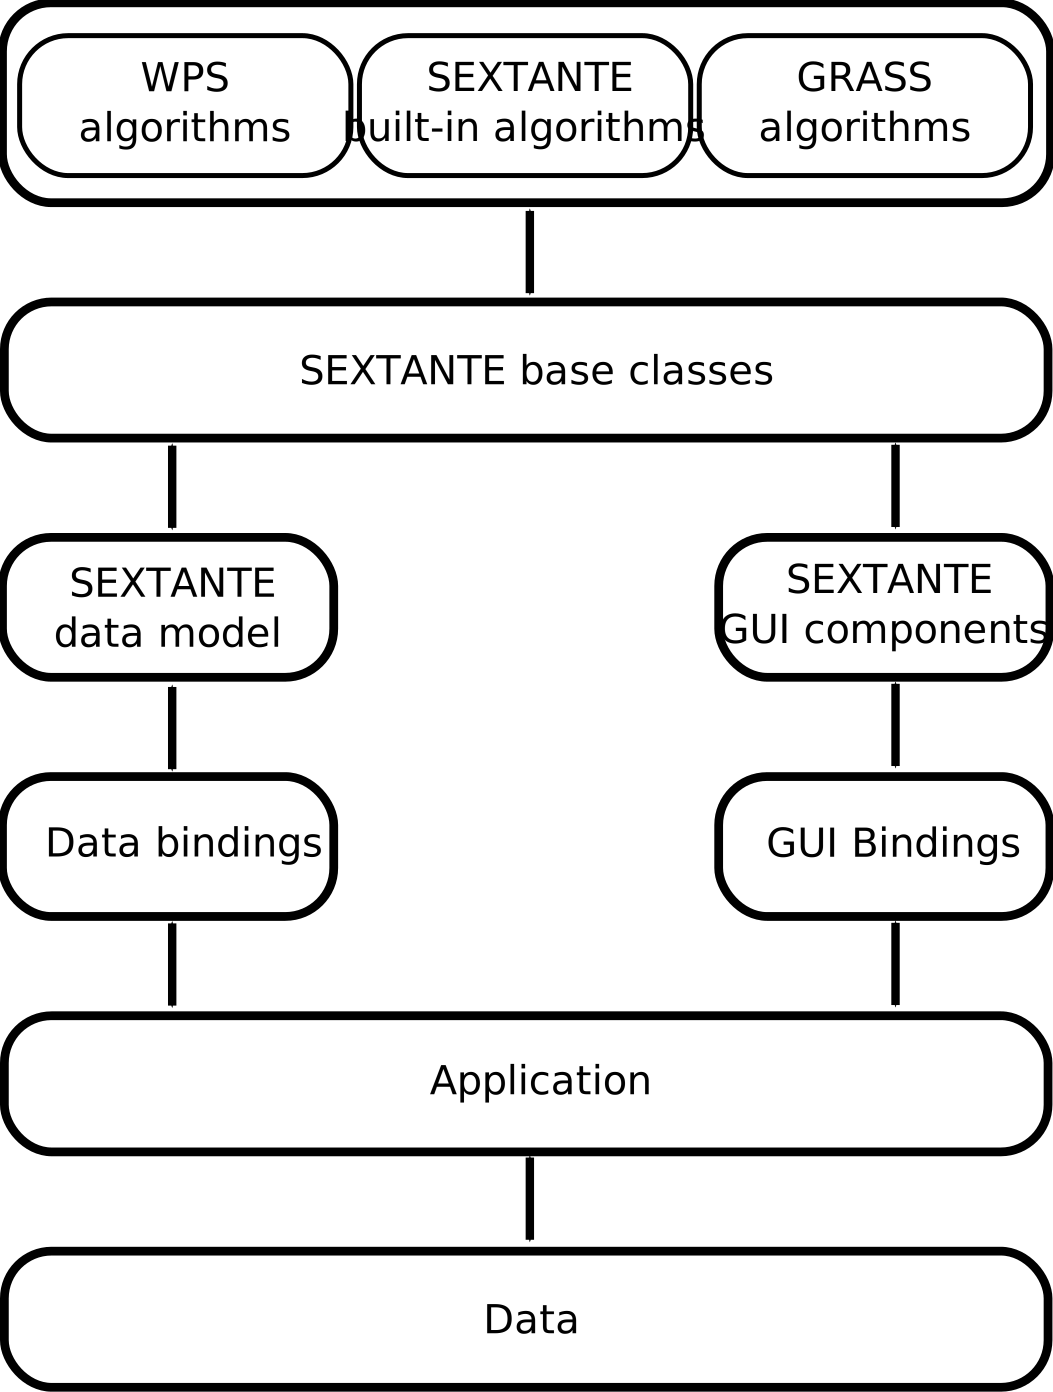
\includegraphics[width=.5\textwidth]{architecture.pdf} 
\end{center}

Data bindings are the mechanism used by SEXTANTE to conect the algorithms to differents data sources. Using this, SEXTANTE can run on many different GIS and can provide geospatial analysis capabilities to different applications, regardless of the data model they use. Some applications are based on popular geodata libraries such as GeoTools, while others have their own classes for accesing data files in both raster and vector format. In any case, SEXTANTE algorithms can be used, as long as bindings between the SEXTANTE data model and the data model used in the application exist.

In this programming guide we will see how to use some of the existing bindings, as well as how to create your own ones for your particular application.

SEXTANTE provides three base interfaces that have to be implemented to allow the algorithms to access the data:

\begin{itemize}
 \item \texttt{IRasterLayer}
\item \texttt{IVectorLayer}
\item \texttt{ITable}
\end{itemize}

This interfaces provides the most common methods that are needed to access data objects (for example, getting the value at a given cell in a raster layer, or a geometry from a vector layer) or create new ones (like setting the value at a given cell or adding a new geometry). These interfaces are designed to be simple and to contain just the basic methods needed for performing analysis, and are not designed as general interfaces for those data types.

SEXTANTE itself does not provide any independent implementation of those interfaces. That means that, if you do not rely on a geodata access library, you cannot run SEXTANTE algorithms, because you are not going to have a way of opening data files and creating data objects.

Bindings are just wrappers for your data objects, and SEXTANTE accesses data \emph{through} them. In this programming guide we will use the GeoTools bindings for the examples, which are available for download from the SEXTANTE website and also from the SVN repository (in the jar file the you have downloaded form the SEXTANTE website you will find a folder named \texttt{bindings}, which includes several bindings, among them the ones to be used with the GeoTools library). That means that you have to use GeoTools to access data sources, and once you have a Java object representing some data element, wrap it with the corresponding SEXTANTE binding, so SEXTANTE algorithms can make use of that data element.

In the next chapter we will see more about bindings and how to use them.

Regarding base classes, it is necessary to have a good understanding of them if you want to implement your own geoalgorithms, but not if you just want to use any of the algorithms already developed. Development of new algorithms is covered in chapter \ref{ProgrammingAlgorithms}.

